\documentclass[tikz,border=10pt]{standalone}
\usepackage{tikz}
\usetikzlibrary{arrows.meta,positioning}

\tikzset{
  concept/.style={draw=blue!70!black, line width=1.2pt, rounded corners=3pt, minimum width=2.8cm, minimum height=1.0cm, align=center, fill=none},
  centerbox/.style={draw=green!50!black, line width=1.2pt, rounded corners=4pt, minimum width=3.6cm, minimum height=1.2cm, align=center, fill=none},
  link/.style={-{Stealth[length=3mm]}, line width=1.2pt, draw=black!70}
}

\begin{document}
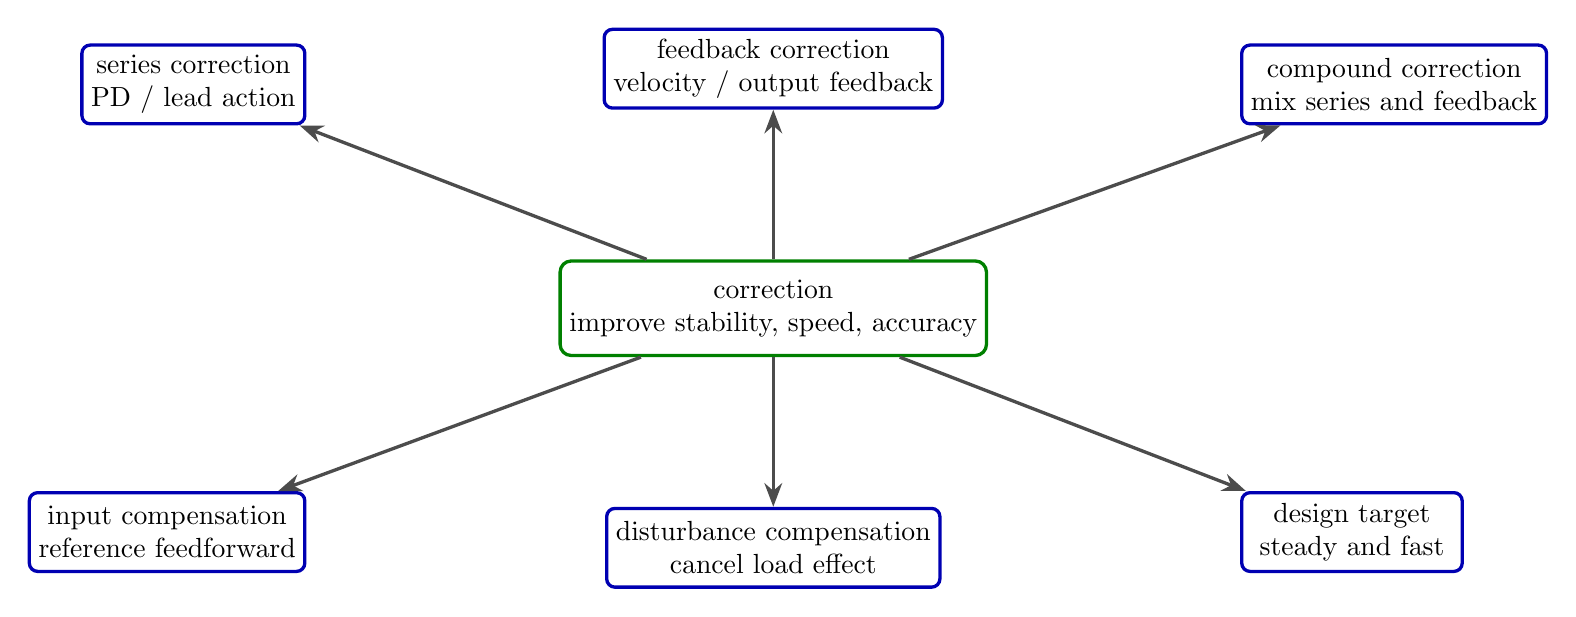
\begin{tikzpicture}[node distance=1.0cm and 1.2cm]
  \node[centerbox] (core) {correction\\improve stability, speed, accuracy};

  \node[concept, above left=1.7cm and 3.2cm of core] (series) {series correction\\PD / lead action};
  \node[concept, above=1.9cm of core] (feedback) {feedback correction\\velocity / output feedback};
  \node[concept, above right=1.7cm and 3.2cm of core] (compound) {compound correction\\mix series and feedback};

  \node[concept, below left=1.7cm and 3.2cm of core] (inputff) {input compensation\\reference feedforward};
  \node[concept, below=1.9cm of core] (disturb) {disturbance compensation\\cancel load effect};
  \node[concept, below right=1.7cm and 3.2cm of core] (target) {design target\\steady and fast};

  \draw[link] (core) -- (series);
  \draw[link] (core) -- (feedback);
  \draw[link] (core) -- (compound);
  \draw[link] (core) -- (inputff);
  \draw[link] (core) -- (disturb);
  \draw[link] (core) -- (target);
\end{tikzpicture}
\end{document}
